\lettrine{A}{n} organization developing a Multi-Tenant software solution, such as a Software as a Service (SaaS), would typically adopt a Microservices Architecture \cite{c2} and likely design the model using a methodology such as Domain-Driven Design \cite{c3}.

Furthermore, the organization must partition the software solution into separate tenants and identities (users and roles). Additionally, it is crucial to assign appropriate permissions to these identities by implementing and associating policies.

It is crucial to note that the Application Development Life Cycle requires distinct and isolated environments for each phase of the development. Therefore, it is imperative to establish multiple environments, such as Development (DEV), User Acceptance Testing (UAT), and Production (PROD).

\begin{figure}[htbp]
    \centering
    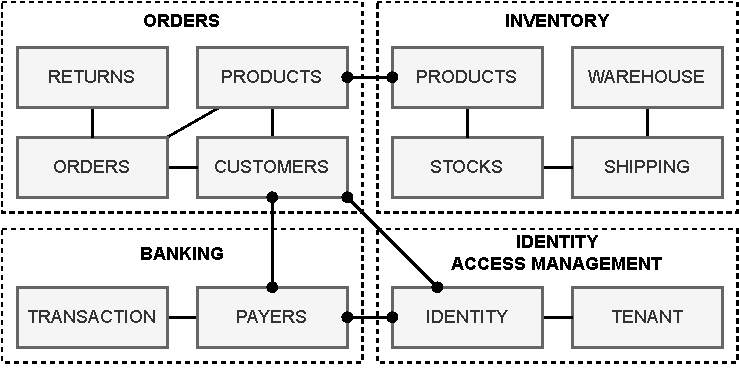
\includegraphics[width=\linewidth]{problem-definition/microservices-ddd-bounded-contexts.pdf}
    \caption{DDD Bounded Contexts}
    \label{fig:microservices-ddd-bounded-contexts}
\end{figure}

Figure \ref{fig:microservices-ddd-bounded-contexts} illustrates an example of bounded contexts using the Domain-Driven Design (DDD) methodology for a hypothetical Software as a Service (SaaS) system that offers Order Management System (OMS) functionalities.

\begin{figure}[htbp]
    \centering
    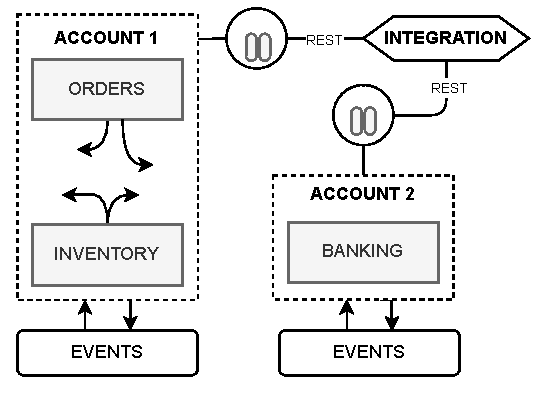
\includegraphics[width=\linewidth]{problem-definition/microservices-architecture.pdf}
    \caption{Microservices Architecture}
    \label{fig:microservices-architecture}
\end{figure}

Meanwhile, Figure \ref{fig:microservices-architecture} depicts a microservices-based architectural solution that employs the proposed Access Control Solution (ACS) approach. This solution divides the software across two distinct yet federated accounts, enabling both isolation and integration.

\vspace{15pt}

Let $D_{acs}$ be the database of the Access Control Solution (ACS) with a set or relations $REL_{acs}$ and a set of attributes $A_{acs}$.
$REL_{acs}$ includes $ACCOUNTS$, $TENANTS$, $PERMISSIONS$ etc.
$A_{acs}$ includes attributes such as $AccountId$, $AccountName$, $PolicyName$ etc from the relations.

\vspace{15pt}

Let $E$ be the set of the environments $E = \{e_1, e_2, \ldots, e_n\}$ and let $AC$ represent the set of the accounts $AC = \{a_1, a_2, \ldots, a_n\}$ within the $D_{acs}$ database.

\vspace{15pt}

It is crucial to note that the organization has to assign each account exclusively to a specific environment otherwise it would raise a security risk.

\begin{boxF}
    \begin{definition}[Account Partitioning for Environments]
        Let $AC$ be the set containing all existing accounts and let $E$ represent the set containing all existing environments, Account Partitioning for Environments is defined as the operation of partitioning the set $AC$ with $E$ using the function $f_{env}$ which is formally defined as:
        \begin{equation*}
            \begin{gathered}
                f_{env}:AC \rightarrow AE | AE \subset AC \times E\\
                f_{env}(a_i) = (a_i, e_m)
            \end{gathered}
            \label{definition:fenv}
        \end{equation*}
        moreover, $AE$ denotes a subset of $AC \times E$ resulting from the Account Partitioning for Environments operation on the set $AC$ where for each account $a_i$, the function $f_{env}(a_i)$ generates an unique pair $(a_i, e_m)$.
        Additionally $\forall a_j \in AC$ there exists a unique $e_n \in E$ such that $(a_j,e_n) \in f_{env}$.
        In conclusion, we can state the equivalence $AE \equiv f_{env}$.
        \label{definition:environments-partitioning}
    \end{definition}
\end{boxF}

The set $AC_i$ is a subset of $AC$ with the property $a_m \in AC_i$ and $a_m \notin AC_j$ where $i \neq j$ and so on, such that:

\begin{align*}
    AC_i = \{ & a \mid a \in AC, \nonumber \\
    & \forall (a_i, e_m) \in f_{env}, (a_j, e_n) \in f_{env} : \nonumber \\
    & \quad (a_i \in AC) \wedge (a_j \in AC) \wedge (e_m = e_n) \}
\end{align*}

and:

\begin{equation*}
    \begin{centering}
        \bigcup_{i=1}^{n = |AC|} AC_i = AC 
    \end{centering}
\end{equation*}

and:

\begin{equation*}
    \begin{centering}
        \forall ACi \in AC, ACj \in AC | (i \neq j \rightarrow ACi \cap ACj = \emptyset)
    \end{centering}
\end{equation*}

\vspace{15pt}

An organization developing the software solution, as illustrated in Figure \ref{fig:microservices-architecture}, has to create multiple environments. 
Assuming three environments as per Table~\ref{table:table-environments} (DEV, TEST, and PROD), each requiring two accounts (one for $ORDERS$, $INENTORY$ and one for $BANKING$), this results in a total necessity of six accounts as per Table~\ref{table:table-accounts} .

\begin{boxF}
    It is important to highlight that the $RELATIONS$ are not normalized in the database just for the sake of simplicity, making the explanation of the proposed solution easier to read.
\end{boxF}

\begin{table}[h]
    \caption{The Relation Environments}
    \label{table:table-environments}
    \begin{center}
    \begin{tabular}{|c|}
    \hline
    Env\\
    \hline
    DEV \\
    \hline
    TEST \\
    \hline
    PROD \\
    \hline
    \end{tabular}
    \end{center}
\end{table}

\begin{table}[h]
    \caption{The Relation Accounts}
    \label{table:table-accounts}
    \begin{center}
    \begin{tabular}{|c|c|c|}
    \hline
    AccountId & AccountName & Env\\
    \hline
    581616507495 & Orders Account & DEV \\
    \hline
    655814852128 & Banking Account & DEV \\
    \hline
    669871239854 & Orders Account & TEST \\
    \hline
    986167786642 & Banking Account & TEST \\
    \hline
    951435799851 & Orders Account & PROD \\
    \hline
    452917331579 & Banking Account & PROD \\
    \hline
    \end{tabular}
    \end{center}
\end{table}

The sets $E$ and $AC$ can be respectively related to the relations $ENVIRONMENTS$ and $ACCOUNTS$ as follows:

\begin{equation*}
    \begin{gathered}
        E = \pi{\{Env\}}(ENVIRONMENTS) \\
        AC = \pi{\{AccountId\}}(ACCOUNTS)
    \end{gathered}
\end{equation*}

\vspace{15pt}

The $ACCOUNTS$ relation has been populated through the Account Partitioning for Environments operation, as defined in Definition~\ref{definition:fenv}.
This implies the existence of three sets, each of which is a subset of $AC$.

\begin{equation*}
    \begin{gathered}
        AC_{dev} = \{581616507495, 655814852128\} \\
        AC_{test} = \{669871239854, 986167786642\} \\
        AC_{prod} = \{951435799851, 452917331579\}
    \end{gathered}
\end{equation*}

\begin{boxF}
    For the sake of simplicity, the following tables will display only the PROD account data to avoid confusion.
\end{boxF}

First step is to configure each account with Projects and Domains, as following:
\begin{itemize}
    \item \textbf{Order Account}: A project named OMS-System and its two domains named Order and Inventory.
    \item \textbf{Banking Account}: A project named Banking-System and its domain named Banking.
\end{itemize}

\begin{table}[h]
    \caption{the relation projects}
    \label{table:table-projects}
    \begin{center}
    \begin{tabular}{|c|c|}
    \hline
    Project & AccountId\\
    \hline
    oms-system & 951435799851 \\
    \hline
    banking-system & 452917331579 \\
    \hline
    \end{tabular}
    \end{center}
\end{table}

\begin{table}[h]
    \caption{the relation domains}
    \label{table:table-domains}
    \begin{center}
    \begin{tabular}{|c|c|c|c|}
    \hline
    Domainid & Domain & Project & AccountId\\
    \hline
    1 & orders & oms-system & 951435799851\\
    \hline
    2 & inventory & oms-system & 951435799851\\
    \hline
    3 & banking & banking-system & 452917331579\\
    \hline
    \end{tabular}
    \end{center}
\end{table}

Each domain then needs to be further partitioned into resources and actions.

\begin{table}[h]
    \caption{the relation resources}
    \label{table:table-resources}
    \begin{center}
    \begin{tabular}{|c|c|}
    \hline
    Resource & DomainId\\
    \hline
    product & 1\\
    \hline
    customer & 1\\
    \hline
    order & 1\\
    \hline
    return & 1\\
    \hline
    product & 2\\
    \hline
    stock & 2\\
    \hline
    warehouse & 2\\
    \hline
    shipping & 2\\
    \hline
    transaction & 3\\
    \hline
    payer & 3\\
    \hline
    \end{tabular}
    \end{center}
\end{table}

\begin{table}[h]
    \caption{the relation actions}
    \label{table:table-actions}
    \begin{center}
    \begin{tabular}{|c|c|c|}
    \hline
    Action & Resource & DomainId\\
    \hline
    get & product & 1\\
    \hline
    upsert & product & 1\\
    \hline
    delete & product & 1\\
    \hline
    get & customer & 1\\
    \hline
    upsert & customer & 1\\
    \hline
    delete & customer & 1\\
    \hline
    get & order & 1\\
    \hline
    upsert & order & 1\\
    \hline
    delete & order & 1\\
    \hline
    get & return & 1\\
    \hline
    upsert & return & 1\\
    \hline
    delete & return & 1\\
    \hline
    get & product & 2\\
    \hline
    upsert & product & 2\\
    \hline
    delete & product & 2\\
    \hline
    get & stock & 2\\
    \hline
    upsert & stock & 2\\
    \hline
    delete & stock & 2\\
    \hline
    get & warehouse & 2\\
    \hline
    upsert & warehouse & 2\\
    \hline
    delete & warehouse & 2\\
    \hline
    get & shipping & 2\\
    \hline
    upsert & shipping & 2\\
    \hline
    delete & shipping & 2\\
    \hline
    get & transaction & 3\\
    \hline
    upsert & transaction & 3\\
    \hline
    softdelete & transaction & 3\\
    \hline
    get & payer & 3\\
    \hline
    upsert & payer & 3\\
    \hline
    softdelete & payer & 3\\
    \hline
    \end{tabular}
    \end{center}
\end{table}

To complete the configurations, it is necessary to create the $TENANTS$ and $IDENTITIES$ relations as per Table~\ref{table:table-tenants}.

\vspace{15pt}

In summary, we've created accounts and environments, established the necessary relations between them. Following that, for each account, projects, domains, resources, and actions were generated. 
Lastly, configurations for tenants and identities were completed.

\begin{table}[h]
    \caption{The Relation Tenants}
    \label{table:table-tenants}
    \begin{center}
    \begin{tabular}{|c|c|}
    \hline
    Tenant & AccountId\\
    \hline
    default & 951435799851 \\
    \hline
    tenant1 & 951435799851 \\
    \hline
    tenant2 & 951435799851 \\
    \hline
    default & 452917331579 \\
    \hline
    tenant1 & 452917331579 \\
    \hline
    tenant2 & 452917331579 \\
    \hline
    \end{tabular}
    \end{center}
\end{table}

\begin{table}[h]
    \caption{The Relation Identities}
    \label{table:table-identities}
    \begin{center}
    \begin{tabular}{|c|c|c|c|c|}
    \hline
    IdentityId & IdentityName & IdentityType & Tenant & Account\\
    \hline
    1 & email-1 & USER & default & 951435799851\\
    \hline
    2 & email-2 & USER & tenant1 & 951435799851\\
    \hline
    3 & email-2 & USER & tenant1 & 452917331579\\
    \hline
    4 & email-2 & USER & tenant2 & 951435799851\\
    \hline
    5 & email-2 & USER & tenant2 & 452917331579\\
    \hline
    6 & platform-manager & ROLE &  default & 951435799851\\
    \hline
    7 & platform-manager & ROLE &  default & 452917331579\\
    \hline
    8 & orders-manager & ROLE &  tenant1 & 951435799851\\
    \hline
    9 & orders-user & ROLE &  tenant1 & 951435799851\\
    \hline
    10 & orders-manager & ROLE &  tenant2 & 951435799851\\
    \hline
    11 & orders-user & ROLE &  tenant2 & 951435799851\\
    \hline
    12 & banking-manager & ROLE & tenant1 & 452917331579\\
    \hline
    13 & banking-user & ROLE & tenant1 & 452917331579\\
    \hline
    14 & banking-manager & ROLE & tenant2 & 452917331579\\
    \hline
    15 & banking-user & ROLE & tenant2 & 452917331579\\
    \hline
    \end{tabular}
    \end{center}
\end{table}

\vspace{15pt}

The Access Control Solution (ACS) helps clearly identify resources and actions by using a UUR (Universally Unique Resource) and RA (Resource Action).

\vspace{15pt}

A UUR is expressed as a string with the specific template:, 
\begin{equation*}
    \begin{gathered}
        \resizebox{.5\textwidth}{!}{%
            uur:\{account\}:\{tenant\}:\{project\}:\{domain\}:\{resource\}/\{resource-filter\}
        }
    \end{gathered}
\end{equation*}

Following is an example of a UUR for the "orders" domain in the project "oms-system" for the "default" tenant, targeting the resource "product" with ID "22":
\begin{equation*}
    \begin{gathered}
        \resizebox{.4\textwidth}{!}{%
            uur:951435799851:default:oms-system:orders:product/22
        }
    \end{gathered}
\end{equation*}

\vspace{15pt}

An AR is expressed as a string with the specific template:, 
\begin{equation*}
    \begin{gathered}
        {resource}:{action}
    \end{gathered}
\end{equation*}

Following is an example of an AR for the action "get" on the resource "product":
\begin{equation*}
    \begin{gathered}
        product:get
    \end{gathered}
\end{equation*}

Both $UUR$ and $UUA$ accept wildcard characters for matching wildcards.

The final step is a set of policies formed by combining the UUR (Universally Unique Resource) and the RA (Resource Action) as per Table~\ref{table:table-policies}.

\begin{table*}[htbp]
    \caption{The Relation Policies}
    \label{table:table-policies}
    \begin{center}
    \begin{tabular}{|c|c|c|c|}
    \hline
    PolicyId & Effect & UUR & UUA\\
    \hline
    p1 & allow & uur:951435799851:tenant1:oms-system:orders:product/* & product:get\\
    \hline
    p2 & allow & uur:951435799851:tenant1:oms-system:orders:order/* & product:create\\
    \hline
    p3 & allow & uur:951435799851:tenant1:oms-system:orders:product/* & order:get\\
    \hline
    p4 & allow & uur:951435799851:tenant1:oms-system:orders:product/* & order:create\\
    \hline
    p5 & allow & uur:452917331579:tenant1:banking-system:transation:* & transation:get\\
    \hline
    p6 & allow & uur:452917331579:tenant1:banking-system:transation:* & transation:create\\
    \hline
    p7 & deny & uur:452917331579:tenant1:banking-system:transation:* & transation:delete\\
    \hline
    \end{tabular}
    \end{center}
\end{table*}

\begin{table*}[htbp]
    \caption{The Relation IdentitiesPolicies}
    \label{table:table-identities-policies}
    \begin{center}
    \begin{tabular}{|c|c|}
    \hline
    IdentityId & PolicyId\\
    \hline
    2 & p1\\
    \hline
    2 & p3\\
    \hline
    2 & p5\\
    \hline
    8 & p1\\
    \hline
    8 & p2\\
    \hline
    8 & p3\\
    \hline
    8 & p4\\
    \hline
    9 & p1\\
    \hline
    9 & p3\\
    \hline
    13 & p5\\
    \hline
    \end{tabular}
    \end{center}
\end{table*}


\newpage

The implemented software solution presents four distinct types of issues.

\subsection{Policies latency and consistency}
\label{sec:policies-latency-consistency}

Evaluating policies on each computing node can be a resource-intensive operation, especially in scenarios with numerous policies. This process is susceptible to both latency and consistency issues, arising from network latencies between nodes and network partitioning.

\subsection{Hacking of the Roles with Messages}
\label{sec:hacking-role-messages}

In a distributed system, a common scenario involves publishing a message that is later consumed by a different node.
The node consuming the message should ideally have identical permissions to the one that published it.

However, if the consuming node has excessively broad permissions, it poses a security risk, potentially executing actions that were not intended to be permitted. 
On the other hand, excessively narrow permissions may prevent the node from executing actions it needs to perform.

These issues need to be addressed both at the message level and the identity level to ensure a balance between security and functionality in the distributed system.

\begin{figure}[h]
    \centering
    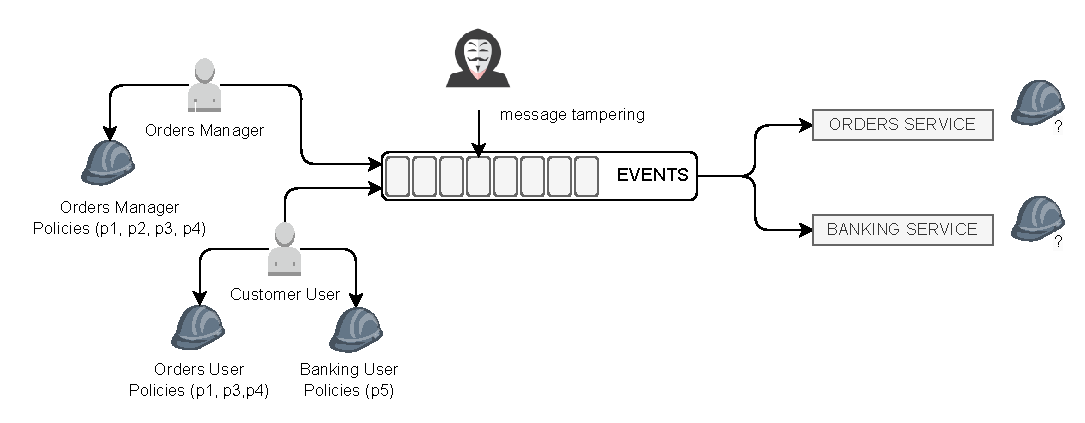
\includegraphics[width=\linewidth]{problem-definition/hacking-role-message.pdf}
    \caption{Hacking of the Roles with Message}
    \label{fig:hacking-roles-messages}
\end{figure}

\subsection{Hacking of the Roles with Messages using Policies is no longer Allowed}
\label{sec:hacking-republish-message}


Especially in an Eventual Consistent system, the time it takes to process an action can be significantly delayed from when it was initially requested. 
This introduces another type of issue where an identity publishes a message that is later consumed by a different identity. 
However, the original identity that published the message no longer has the permission to execute that action.

In such cases, the system should either discard the message without processing it or redirect the message to a different queue, necessitating an approval process.

Similar to the previous issue, this challenge can be tackled at both the message level and the identity level to maintain a balance between security and functionality in the system.

\begin{figure}[h]
    \centering
    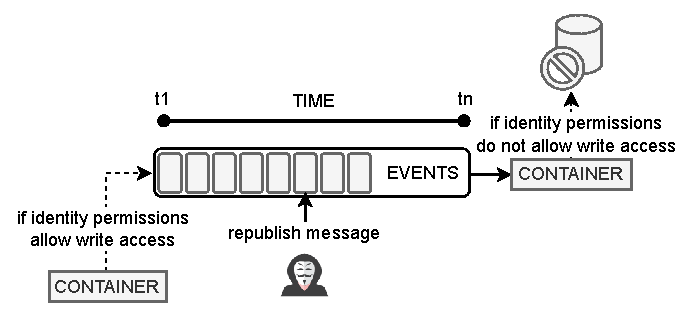
\includegraphics[width=\linewidth]{problem-definition/hacking-republish-message.pdf}
    \caption{Hacking of the Roles with Messages using Policies are no longer Allowed}
    \label{fig:hacking-republish-message}
\end{figure}

\subsection{Risk of complex policies evaluation}
\label{sec:policies-evaluation-risk}

Evaluating complex policies at runtime raises security concerns because unforeseen situations may lack protection, leading to a potential risk of an attack. 
Therefore, having a system in place to prevent such attacks is crucial, and one effective approach is to assess the system's security by generating risk scores.
